\chapter{Quando usar cada teste?}

\section{Provocação: como comparar grupos e avaliar relações entre variáveis?}

No estudo FIRE AND ICE, os pesquisadores compararam duas técnicas de ablação
para fibrilação atrial: crioablação por balão e ablação por radiofrequência.
A pergunta principal do estudo era se as duas estratégias apresentavam eficácia
comparável dentro de uma margem de não inferioridade previamente definida.

Além do desfecho principal, os dados permitem formular perguntas estatísticas
mais simples e fundamentais:

\begin{itemize}
    \item A idade dos participantes é semelhante nos dois grupos?
    \item A proporção de homens difere entre os grupos?
    \item O tempo médio de procedimento difere entre os tratamentos?
    \item Existe associação entre idade e pressão arterial?
    \item Existe associação entre o grupo de tratamento e uma complicação?
    \item Como comparar três ou mais grupos quando a variável de interesse é quantitativa?
\end{itemize}

Essas perguntas envolvem principalmente duas ideias:

\begin{itemize}
    \item \textbf{comparação:} investigar se uma variável apresenta valores ou
    distribuições diferentes entre grupos;
    \item \textbf{associação:} investigar se os valores ou categorias de uma
    variável estão relacionados aos de outra.
\end{itemize}

Um resultado estatisticamente não significativo não demonstra que não exista
qualquer diferença ou associação. Significa que, sob o modelo e as hipóteses
adotados, os dados não forneceram evidência estatística suficiente para
rejeitar a hipótese nula.

Da mesma forma, um resultado estatisticamente significativo não informa, por
si só, se o efeito é grande, clinicamente importante ou causal.

\section{Testes para uma média}

Quando existe uma única amostra e a pergunta é comparar sua média com um valor
de referência, podemos utilizar um teste para uma média.

\subsection{Teste-t de uma amostra}

O teste-$t$ de uma amostra é apropriado quando queremos avaliar se a média
populacional difere de um valor de referência $\mu_0$, especialmente quando
o desvio-padrão populacional é desconhecido.

As hipóteses, em um teste bilateral, são:

\begin{itemize}
    \item $H_0:\mu=\mu_0$;
    \item $H_1:\mu\neq\mu_0$.
\end{itemize}

A estatística de teste é:

\begin{equation}
  t= \frac{\bar X-\mu_0}{s/\sqrt{n}}
\end{equation}

com:

\begin{equation}
  gl=n-1.
\end{equation}

O teste pressupõe, principalmente, independência das observações e, em
amostras pequenas, distribuição aproximadamente normal da variável na
população. Em amostras maiores, o teste pode ser bastante robusto a desvios
moderados da normalidade, embora valores extremos e forte assimetria ainda
possam ser problemáticos.

Em R, o procedimento pode ser realizado com:

\begin{code}[Código: teste-$t$ de uma amostra]
resultado_t1 <-
  t.test(
    x = dados$pressao,
    mu = 120,
    alternative = "two.sided"
  )

resultado_t1
\end{code}

O intervalo de confiança da média fornece informação complementar ao
valor-$p$ e deve ser considerado na interpretação.

\subsection{Teste-z para uma média}

O teste-$z$ para uma média utiliza a distribuição normal padrão e pressupõe
que o desvio-padrão populacional $\sigma$ seja conhecido:

\begin{equation}
  z= \frac{\bar X-\mu_0}{\sigma/\sqrt{n}}.
\end{equation}

Na prática, essa situação é relativamente incomum em aplicações biomédicas.
Quando $\sigma$ é desconhecido e precisa ser estimado pela amostra, o
teste-$t$ é geralmente o procedimento apropriado.

Por isso, embora o teste-$z$ seja importante para compreender a teoria dos
testes de hipóteses, o teste-$t$ é muito mais comum na prática quando estamos
comparando uma média com um valor de referência.

\section{Comparação de duas médias}

Quando a variável de interesse é quantitativa e existem dois grupos, a
primeira pergunta a ser feita é se as observações são independentes ou
pareadas.

\subsection{Teste-t de Student pareado}

O teste-$t$ pareado é utilizado quando duas observações estão naturalmente
relacionadas.

Exemplos incluem:

\begin{itemize}
    \item medidas antes e depois no mesmo paciente;
    \item duas medidas obtidas do mesmo indivíduo;
    \item participantes explicitamente emparelhados por um desenho de estudo.
\end{itemize}

Para cada par, calcula-se:

\begin{equation}
  d_i=\text{depois}_i-\text{antes}_i.
\end{equation}

A análise é então equivalente a realizar um teste-$t$ de uma amostra sobre
as diferenças.

A estatística é:

\begin{equation}
  t=
  \frac{\bar d}
  {s_d/\sqrt{n}}
\end{equation}

em que $\bar d$ é a média das diferenças, $s_d$ é o desvio-padrão das
diferenças e $n$ é o número de pares.

As hipóteses são:

\begin{itemize}
    \item $H_0:\mu_d=0$;
    \item $H_1:\mu_d\neq0$.
\end{itemize}

Os graus de liberdade são:

\[
gl=n-1.
\]

\begin{deepdive}
\boxtitle{Pressupostos do teste-$t$ pareado}
O principal pressuposto de distribuição refere-se às \textbf{diferenças}
$d_i$, e não às duas variáveis consideradas separadamente.

Os principais aspectos são:

\begin{itemize}
    \item diferenças aproximadamente normais em amostras pequenas;
    \item independência entre os pares;
    \item pareamento correto das observações;
    \item variável quantitativa cuja diferença tenha interpretação científica.
\end{itemize}

Quando esses pressupostos não são adequados, pode-se considerar o teste de
Wilcoxon para postos sinalizados, desde que a pergunta científica seja
compatível com um procedimento baseado em postos.
\end{deepdive}

\subsection{Teste-t para duas amostras independentes}

Quando a variável de interesse é quantitativa e existem dois grupos
independentes, uma possibilidade é comparar suas médias.

O teste-$t$ clássico para duas amostras independentes assume variâncias
populacionais iguais. Se os grupos possuem variâncias populacionais iguais, a estimativa agrupada
da variância é:

\begin{equation}
  s_p^2=
  \frac{
  (n_1-1)s_1^2+(n_2-1)s_2^2
  }{
  n_1+n_2-2
  }
\end{equation}

A estatística de teste é:

\begin{equation}
  t=
  \frac{\bar X_1-\bar X_2}
  {s_p\sqrt{\frac{1}{n_1}+\frac{1}{n_2}}}
\end{equation}

com:

\begin{equation}
  gl=n_1+n_2-2
\end{equation}

As hipóteses para um teste bilateral são:

\begin{itemize}
    \item $H_0:\mu_1=\mu_2$;
    \item $H_1:\mu_1\neq\mu_2$.
\end{itemize}

A diferença entre as médias deve ser apresentada juntamente com seu intervalo
de confiança. O valor de $p$ informa a evidência contra a hipótese nula, mas
não informa sozinho a magnitude ou a importância clínica da diferença.

\subsection{Teste-t de Welch}

O teste de Welch é uma alternativa ao teste-$t$ com variâncias agrupadas e
não exige igualdade das variâncias populacionais.

Sua estatística é:

\begin{equation}
  t=
\frac{\bar X_1-\bar X_2}
{\sqrt{\frac{s_1^2}{n_1}+\frac{s_2^2}{n_2}}}
\end{equation}

Os graus de liberdade são aproximados pela fórmula de Welch--Satterthwaite:

\begin{equation}
gl \approx
\frac{
\left(
\frac{s_1^2}{n_1}+
\frac{s_2^2}{n_2}
\right)^2
}{
\frac{
(s_1^2/n_1)^2
}{n_1-1}
+
\frac{
(s_2^2/n_2)^2
}{n_2-1}
}
\end{equation}

Como não exige variâncias iguais e apresenta bom desempenho em uma ampla
variedade de situações, o teste de Welch é frequentemente uma escolha padrão
para a comparação de duas médias independentes.

\begin{deepdive}[]
\boxtitle{Uma observação importante sobre os testes de variância}
Não é necessário realizar obrigatoriamente um teste de igualdade das variâncias
antes de escolher entre o teste-$t$ clássico e o teste de Welch. Na prática, Welch pode ser utilizado diretamente como análise principal, pois
evita a necessidade de tomar uma decisão baseada em um teste preliminar de
variâncias. Quando os tamanhos amostrais são semelhantes e as variâncias também são
semelhantes, os resultados dos dois procedimentos tendem a ser muito próximos.
\end{deepdive}

\begin{deepdive}
\boxtitle{Comparação de mais de duas médias}
Quando se deseja comparar médias de três ou mais grupos, realizar muitos
testes-$t$ separadamente aumenta a probabilidade de pelo menos um falso
positivo.

A análise de variância, ou ANOVA, fornece um teste global para a hipótese de
igualdade das médias.

As hipóteses são:

\begin{itemize}
    \item $H_0:\mu_1=\mu_2=\cdots=\mu_k$;
    \item $H_1$: pelo menos uma das médias difere.
\end{itemize}

Um resultado significativo indica que nem todas as médias são iguais. Ele não
identifica quais grupos diferem. Para investigar comparações específicas, devem ser utilizados procedimentos
pós-hoc ou contrastes planejados com controle adequado do erro decorrente de
múltiplas comparações.

Os principais pressupostos da ANOVA clássica são:

\begin{itemize}
    \item independência das observações;
    \item resíduos aproximadamente normais;
    \item variâncias aproximadamente iguais entre os grupos;
    \item ausência de valores extremos com influência desproporcional.
\end{itemize}

Quando as variâncias diferem, a ANOVA de Welch pode ser utilizada. Quando os dados são ordinais ou as condições para uma análise baseada em médias são muito inadequadas, o teste de Kruskal--Wallis pode ser considerado.
\end{deepdive}

\section{Associação entre duas variáveis categóricas}

\subsection{Teste qui-quadrado de independência}

O teste qui-quadrado de independência avalia a hipótese de que duas variáveis
categóricas são independentes na população.

\begin{definition}[Teste qui-quadrado de independência]

Para uma tabela com $r$ linhas e $c$ colunas:

\begin{itemize}
    \item $H_0$: as variáveis são independentes;
    \item $H_1$: as variáveis não são independentes.
\end{itemize}

As frequências esperadas são:

\begin{equation}
  E_{ij}
=
\frac{
(\text{total da linha }i)
(\text{total da coluna }j)
}{
\text{total geral}
}
\end{equation}

A estatística é:


\begin{equation}
\chi^2=
\sum_{i=1}^{r}\sum_{j=1}^{c}
\frac{(O_{ij}-E_{ij})^2}{E_{ij}}
\end{equation}

com:

\begin{equation}
gl=(r-1)(c-1)
\end{equation}

\end{definition}

Um resultado significativo fornece evidência de associação entre as variáveis,
mas não informa automaticamente a magnitude ou a importância clínica dessa
associação.

Para interpretar a associação, é importante observar as proporções e, quando
apropriado, medidas de efeito como diferença de riscos, razão de riscos,
razão de prevalências ou odds ratio.

\subsection{Pressupostos do qui-quadrado}

O teste pressupõe:

\begin{itemize}
    \item observações independentes;
    \item cada indivíduo contribuindo para uma única célula da tabela;
    \item frequências esperadas suficientemente grandes para que a aproximação
    qui-quadrado seja adequada.
\end{itemize}

Não existe uma única regra universal para ``frequência esperada mínima''. Uma
regra prática frequentemente utilizada é que as frequências esperadas sejam
pelo menos 5, mas critérios mais flexíveis podem ser adequados dependendo do
tamanho e da estrutura da tabela.

Quando as contagens esperadas são pequenas, métodos exatos ou métodos de
simulação podem ser preferíveis. Categorias não devem ser agrupadas apenas para satisfazer uma regra estatística. O agrupamento precisa ter justificativa científica e preservar uma interpretação coerente.

\subsection{Teste exato de Fisher}

Em tabelas $2\times2$ com contagens pequenas, o teste exato de Fisher é uma
alternativa importante. Ele calcula a probabilidade de observar tabelas tão ou mais extremas que a observada, condicionando aos totais marginais. 

Para tabelas maiores, podem ser considerados métodos exatos ou simulações de
Monte Carlo, dependendo do problema e do software utilizado.

\begin{error}
\boxtitle{Como interpretar um resultado do qui-quadrado}
Um valor de $p\geq0.05$ não prova que as variáveis sejam independentes. Indica
apenas que os dados não forneceram evidência estatística suficiente para
rejeitar a hipótese de independência.

Da mesma forma, um resultado significativo não informa sozinho a importância
da associação.

A interpretação deve considerar:

\begin{itemize}
    \item proporções observadas;
    \item diferença absoluta entre proporções;
    \item medida de efeito apropriada;
    \item intervalo de confiança;
    \item contexto clínico.
\end{itemize}
\end{error}

\section{Correlação de Pearson}

A correlação de Pearson é uma medida utilizada para quantificar a intensidade
e a direção da associação \textbf{linear} entre duas variáveis quantitativas.
Ela é especialmente útil quando a pergunta científica é se valores maiores
de uma variável tendem a estar associados a valores maiores ou menores da
outra.

O coeficiente de correlação populacional é denotado por $\rho$, enquanto sua
estimativa na amostra é representada por $r$. O coeficiente amostral é
definido por:

\begin{equation}
  r=
\frac{
\displaystyle\sum_{i=1}^{n}
(x_i-\bar{x})(y_i-\bar{y})
}{
\sqrt{
\displaystyle\sum_{i=1}^{n}(x_i-\bar{x})^2
\displaystyle\sum_{i=1}^{n}(y_i-\bar{y})^2
}
}
\end{equation}

O coeficiente sempre assume valores entre $-1$ e $1$. Valores positivos indicam que valores maiores de $X$ tendem a estar associados
a valores maiores de $Y$, enquanto valores negativos indicam que valores
maiores de $X$ tendem a estar associados a valores menores de $Y$.

Um valor de $r$ próximo de zero indica ausência de associação \textbf{linear}. Isso não significa necessariamente que não exista qualquer relação entre as variáveis. Uma relação fortemente não linear, por exemplo, pode apresentar correlação de Pearson próxima de zero.

\begin{deepdive}
\boxtitle{A importância do gráfico de dispersão}

O coeficiente de Pearson resume toda a relação entre duas variáveis em um
único número. Por isso, duas situações muito diferentes podem produzir
valores semelhantes de $r$.

Antes de calcular e interpretar a correlação, é recomendável construir um
gráfico de dispersão. Esse gráfico permite verificar:

\begin{itemize}
    \item se a relação é aproximadamente linear;
    \item se existem valores extremos;
    \item se a variabilidade de $Y$ muda ao longo dos valores de $X$;
    \item se existem grupos distintos de observações;
    \item se a associação parece ser determinada por poucas observações.
\end{itemize}

Assim, o valor de $r$ não deve ser interpretado isoladamente. A representação
gráfica é uma etapa importante da análise exploratória.
\end{deepdive}

\subsection{Teste de significância da correlação}

Quando o objetivo é testar estatisticamente a existência de associação linear
na população, podemos formular as hipóteses:


Para um teste bilateral, a estatística de teste pode ser calculada por:


\begin{equation}
  t=
\frac{
r\sqrt{n-2}
}{
\sqrt{1-r^2}
}
\end{equation}


que, sob a hipótese nula e sob as condições apropriadas, segue uma
distribuição $t$ de Student com:


\begin{equation}
  t= gl=n-2
\end{equation}

Um valor-$p$ pequeno fornece evidência estatística contra a hipótese de que
a correlação linear populacional seja igual a zero.

Entretanto, o valor-$p$ não informa a magnitude da associação. Uma amostra
muito grande pode produzir um valor-$p$ pequeno para uma correlação de pequena
magnitude. Por esse motivo, a interpretação deve considerar conjuntamente:

\begin{itemize}
    \item o valor de $r$;
    \item o intervalo de confiança para $\rho$;
    \item o valor-$p$;
    \item o gráfico de dispersão;
    \item a relevância científica da associação.
\end{itemize}

\subsection{Pressupostos e condições de uso}

A correlação de Pearson deve ser utilizada quando a relação de interesse é
linear e as observações são independentes.

Um aspecto importante é que a \textbf{normalidade não deve ser avaliada
simplesmente exigindo que cada variável, isoladamente, tenha distribuição
normal}. Para a inferência clássica do teste de Pearson, a formulação teórica
mais forte envolve a distribuição conjunta aproximadamente normal das duas
variáveis.

\subsection{Valores extremos e observações influentes}

A correlação de Pearson pode ser bastante sensível a valores extremos.
Uma única observação distante das demais pode alterar substancialmente o valor
de $r$ e, consequentemente, o resultado do teste de significância.

Por esse motivo, a análise deve investigar a presença de observações
potencialmente influentes. Um gráfico de dispersão é particularmente útil
para essa finalidade.

Quando valores extremos são identificados, eles não devem ser simplesmente
removidos para produzir uma correlação mais conveniente. É necessário
investigar sua origem e verificar se representam erros de medição, registros
incorretos ou observações reais da população estudada.

\subsection{Interpretação}

Não existe uma classificação universal segundo a qual determinado intervalo
de valores de $r$ seja automaticamente ``fraco'', ``moderado'' ou ``forte''.
A magnitude considerada relevante depende do contexto científico, da área de
aplicação e da finalidade da análise.

Uma correlação de $r=0{,}20$ pode ser relevante em determinado contexto,
enquanto uma correlação de $r=0{,}80$ pode ser pouco informativa em outro.

Assim, uma interpretação adequada deve evitar frases como ``a correlação foi
significativa, portanto as variáveis estão fortemente relacionadas''. O
resultado deve ser descrito considerando simultaneamente a magnitude, a
incerteza e o contexto científico.

Por exemplo, uma forma adequada de apresentar um resultado seria:

\begin{quote}
Foi observada uma correlação linear positiva entre as duas variáveis
($r=0{,}55$; IC 95\%: $0{,}50$--$0{,}60$; $p<0{,}001$), indicando que valores
maiores de uma variável tendem a estar associados a valores maiores da outra.
\end{quote}

Essa formulação descreve a associação sem transformá-la indevidamente em uma
relação causal.

\section{Implementação em R}

\subsection{Preparação dos dados}

O exemplo a seguir utiliza dados simulados para ilustrar a implementação dos
métodos. Eles não devem ser confundidos com os dados individuais originais do
estudo FIRE AND ICE.

\begin{code}[Código: carregar pacotes e criar dados simulados]
# Carregar pacotes necessários
library(tidyverse)

# Tornar a simulação reproduzível
set.seed(123)

# Criar dataset simulado
fire_ice <- data.frame(
  id = 1:750,
  grupo = rep(c("RF", "Cryo"), c(376, 374)),

  # Tempo de procedimento, em minutos
  tempo_procedimento = c(
    rnorm(376, mean = 142.1, sd = 38.9),
    rnorm(374, mean = 124.7, sd = 32.9)
  ),

  # Evento raro: paralisia do nervo frênico
  paralisia_frenica = c(
    rep("Não", 376),
    sample(
      c(rep("Sim", 8), rep("Não", 374 - 8))
    )
  )
)

# Converter grupo para fator
fire_ice$grupo <- factor(fire_ice$grupo)

# Criar tempo de fluoroscopia
fire_ice$tempo_fluoroscopia <-
  6 +
  0.14 * fire_ice$tempo_procedimento +
  rnorm(750, mean = 0, sd = 5.5)

# Inspecionar estrutura
str(fire_ice)

# Sumário por grupo
fire_ice %>%
  group_by(grupo) %>%
  summarise(
    n = n(),
    tempo_proc_mean = mean(tempo_procedimento),
    tempo_proc_sd = sd(tempo_procedimento),
    frenica_pct =
      mean(paralisia_frenica == "Sim") * 100,
    tempo_fluoro_mean =
      mean(tempo_fluoroscopia)
  )
\end{code}

\subsection{Comparação de duas médias: tempo de procedimento}

Neste exemplo, queremos comparar o tempo médio de procedimento entre RF e
Cryo. Como os grupos são independentes e não há necessidade de assumir variâncias iguais, utilizaremos diretamente o teste-$t$ de Welch.

\begin{code}[Teste-t de Welch]
resultado_t <-
  t.test(
    tempo_procedimento ~ grupo,
    data = fire_ice,
    var.equal = FALSE
  )

resultado_t
\end{code}

O R utiliza o teste de Welch por padrão quando
\texttt{var.equal = FALSE}.

\begin{code}[Resultado]
  	Welch Two Sample t-test

data:  tempo_procedimento by grupo
t = -7.3486, df = 735.22, p-value = 5.34e-13
alternative hypothesis: true difference in means between group Cryo and group RF is not equal to 0
95 percent confidence interval:
 -24.05994 -13.91490
sample estimates:
mean in group Cryo   mean in group RF 
          124.3851           143.3725 
\end{code}

O teste fornece um valor de $p$ muito pequeno
($p = 5{,}34\times10^{-13}$). Portanto, rejeitamos a hipótese nula de
igualdade das médias ao nível de significância de $5\%$. Há forte evidência
estatística de que os tempos médios de procedimento diferem entre os grupos.

O intervalo de confiança de $95\%$ para a diferença entre as médias é:

\[
IC_{95\%} = (-24{,}06,\,-13{,}91)\text{ minutos}.
\]

Como todo o intervalo está abaixo de zero, os dados são compatíveis com um
tempo médio menor no grupo Cryo. Além disso, o intervalo sugere que a
diferença média na população está entre aproximadamente $13{,}9$ e
$24{,}1$ minutos, com Cryo apresentando menor tempo de procedimento.

É importante observar que o intervalo de confiança fornece mais informação
do que o valor-$p$ isoladamente: além de indicar evidência de diferença,
ele fornece uma estimativa da magnitude dessa diferença e de sua incerteza.

Podemos também obter a diferença de médias diretamente:

\begin{code}[Médias por grupo]
fire_ice %>%
  group_by(grupo) %>%
  summarise(
    media = mean(tempo_procedimento),
    desvio_padrao = sd(tempo_procedimento),
    n = n()
  )
\end{code}

A média do tempo de procedimento foi de aproximadamente $124{,}4$ minutos
no grupo Cryo e $143{,}4$ minutos no grupo RF. A diferença observada entre
as médias é, portanto, de aproximadamente:

\[
124{,}39 - 143{,}37 = -18{,}98\text{ minutos}.
\]

Em termos absolutos, o procedimento durou em média cerca de $19$ minutos
a menos no grupo Cryo. Os desvios-padrão, de aproximadamente $32{,}9$ e
$37{,}7$ minutos, mostram que existe variabilidade considerável no tempo de
procedimento dentro de cada grupo.

Assim, neste exemplo, podemos resumir o resultado da seguinte forma: o tempo
médio de procedimento foi menor no grupo Cryo do que no grupo RF, com uma
diferença estimada de aproximadamente $19$ minutos
($IC_{95\%}: 13{,}9$ a $24{,}1$ minutos a favor de Cryo). O valor-$p$
extremamente pequeno fornece forte evidência estatística contra a hipótese
de igualdade das médias

\begin{table}[ht]
\centering
\caption{Média, desvio-padrão e tamanho da amostra por grupo}
\begin{tabularx}{0.8\textwidth}{lXXX}
\toprule
\textbf{Grupo} & \textbf{Média} & \textbf{Desvio-padrão} & \textbf{$n$} \\
\midrule
Cryo & 124,39 & 32,87 & 374 \\
RF   & 143,37 & 37,73 & 376 \\
\bottomrule
\end{tabularx}
\end{table}

\begin{error}
\boxtitle{Dados simulados não são evidência clínica}

Os dados deste exemplo foram gerados artificialmente com \texttt{rnorm()}.
Portanto, o valor de $p$ e o intervalo de confiança descrevem a simulação,
e não constituem uma nova análise do ensaio clínico FIRE AND ICE.

A interpretação clínica de que uma diferença de determinado número de
minutos é importante também deve ser fundamentada em conhecimento clínico,
não apenas no resultado estatístico.
\end{error}

\subsection{Associação entre grupo e paralisia do nervo frênico}

Agora queremos investigar a associação entre grupo de tratamento e ocorrência
de paralisia do nervo frênico. Para fins didáticos, foram simulados oito eventos exclusivamente no grupo Cryo, de modo a ilustrar o comportamento de uma tabela 2x2 com uma célula igual a zero a fim de simplificar o entedimento.

Primeiro construímos a tabela:

\begin{code}[Código: tabela de contingência]
tabela_frenica <-
  table(
    fire_ice$grupo,
    fire_ice$paralisia_frenica
  )

tabela_frenica
\end{code}

O resultado é:

\begin{code}[Tabela observada]
      Não Sim
Cryo  366   8
RF    376   0
\end{code}

Como há uma célula com zero eventos e as frequências esperadas são pequenas,
a aproximação qui-quadrado não é adequada. Caso tentemos rodar a análise, o próprio R retorna um erro porque algumas frequências esperadas são pequenas.

\begin{code}[Qui-quadrado]
resultado_chi <-
  chisq.test(tabela_frenica)
\end{code}

\begin{code}[Resultado qui-quadrado]
Warning in chisq.test(tabela_frenica) :
  Aproximação do qui-quadrado pode estar incorreta
\end{code}

Nesse cenário, utilizaremos o teste exato de Fisher:

\begin{code}[Código: teste exato de Fisher]
resultado_fisher <-
  fisher.test(tabela_frenica)

resultado_fisher
\end{code}

O resultado simulado é aproximadamente:

\begin{code}[Resultado do teste exato de Fisher]
	Fisher's Exact Test for Count Data

data:  tabela_frenica
p-value = 0.003681
alternative hypothesis: true odds ratio is not equal to 1
95 percent confidence interval:
 0.000000 0.575794
sample estimates:
odds ratio 
         0 
\end{code}

O teste exato de Fisher apresentou um valor de $p=0{,}003681$. Como esse
valor é menor que o nível de significância adotado ($\alpha=0{,}05$),
rejeitamos a hipótese nula de ausência de associação entre o grupo de
tratamento e a ocorrência de paralisia do nervo frênico.

Em outras palavras, os dados simulados fornecem evidência estatística de que
a ocorrência de paralisia do nervo frênico está associada ao grupo de
tratamento. Além disso, foi apresentado o conceito de odds ratio, mas este será ignorado por fugir do escopo do manual.

\subsection{Correlação entre tempo de procedimento e fluoroscopia}

Agora investigaremos a associação entre duas variáveis quantitativas:

\begin{itemize}
    \item tempo de procedimento;
    \item tempo de fluoroscopia.
\end{itemize}

Primeiro devemos visualizar a relação.

\begin{code}[Gráfico de dispersão]
ggplot(
  fire_ice,
  aes(
    x = tempo_procedimento,
    y = tempo_fluoroscopia,
    color = grupo
  )
) +
  geom_point(alpha = 0.5) +
  geom_smooth(
    method = "lm",
    se = FALSE
  ) +
  labs(
    title =
      "Tempo de Procedimento vs. Tempo de Fluoroscopia",
    x = "Tempo de procedimento (min)",
    y = "Tempo de fluoroscopia (min)"
  ) +
  theme_minimal()
\end{code}

\begin{figure}[ht]
    \centering
    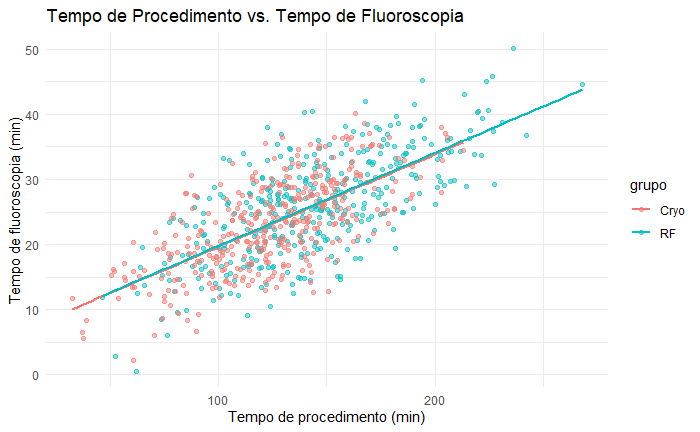
\includegraphics[width=0.8\textwidth]{img/quando.scatter.png}
    \caption{Relação entre tempo de procedimento e tempo de fluoroscopia.}
    \label{fig:scatter_plot}
\end{figure}

O gráfico sugere uma relação linear positiva: procedimentos mais longos
tendem a apresentar também maior tempo de fluoroscopia.

Podemos quantificar essa associação utilizando a correlação de Pearson:

\begin{code}[Código: correlação de Pearson]
resultado_cor <-
  cor.test(
    fire_ice$tempo_procedimento,
    fire_ice$tempo_fluoroscopia,
    method = "pearson"
  )

resultado_cor
\end{code}

O resultado da simulação é:

\begin{code}[Resultado da correlação]
	Pearson's product-moment correlation

data:  fire_ice$tempo_procedimento and fire_ice$tempo_fluoroscopia
t = 26.321, df = 748, p-value < 2.2e-16
alternative hypothesis: true correlation is not equal to 0
95 percent confidence interval:
 0.6543224 0.7288373
sample estimates:
      cor 
0.6934294 
\end{code}

O coeficiente de correlação estimado é:

\[
r = 0{,}693.
\]

O valor positivo indica que as duas variáveis tendem a aumentar juntas.
A magnitude do coeficiente indica uma associação linear positiva de
moderada a forte intensidade no contexto desta simulação.

O intervalo de confiança de $95\%$ para a correlação é aproximadamente:

\[
IC_{95\%} = (0{,}654,\;0{,}729).
\]

Isso indica que, sob as condições do modelo utilizado, os valores
compatíveis com os dados para a correlação populacional estão concentrados
em uma faixa positiva. O intervalo também fornece uma medida da incerteza
associada à estimativa de $r$.

O teste apresenta $p < 2{,}2\times10^{-16}$. Como esse valor é muito menor
que $0{,}05$, rejeitamos a hipótese nula de ausência de correlação linear.
Há, portanto, forte evidência estatística de uma associação linear entre o
tempo de procedimento e o tempo de fluoroscopia nesta simulação.

\begin{error}
\boxtitle{Correlação não é uma relação causal}

Mesmo quando $r$ é elevado e o valor de $p$ é muito pequeno, não podemos
concluir automaticamente que o aumento do tempo de procedimento cause o
aumento do tempo de fluoroscopia.

Neste exemplo, ambas as variáveis podem refletir a complexidade do
procedimento. Além disso, o tempo de fluoroscopia pode depender de fatores
como tecnologia disponível, experiência da equipe e estratégia utilizada.

Portanto, a correlação descreve uma associação observada nos dados simulados.
Ela não estabelece um mecanismo causal.
\end{error}

\begin{deepdive}
\boxtitle{Associação global pode esconder diferenças entre grupos}
Quando os dados pertencem a diferentes grupos, uma correlação calculada
considerando todos os participantes pode misturar fenômenos distintos.

Por exemplo, se RF e Cryo tiverem tempos médios de procedimento diferentes,
parte da associação global entre tempo de procedimento e fluoroscopia pode
estar relacionada simplesmente à diferença entre os grupos.

Por isso, em análises mais avançadas, pode ser útil:

\begin{itemize}
    \item colorir os pontos por grupo;
    \item calcular associações dentro de cada grupo;
    \item utilizar regressão para ajustar pelo grupo;
    \item investigar possíveis interações.
\end{itemize}

Esse problema é um exemplo de por que uma medida de associação isolada nem
sempre responde completamente à pergunta científica.
\end{deepdive}

\section{Como escolher o teste?}

A escolha do teste pode ser organizada a partir da pergunta científica e da
estrutura dos dados.

\begin{table}[htbp]
\centering
\caption{Guia inicial para escolha do procedimento estatístico}
\label{tab:escolha_teste}
\vspace{2mm}

\begin{tabular}{p{4.2cm} p{4.0cm} p{4.5cm}}
\toprule
\textbf{Pergunta} &
\textbf{Estrutura dos dados} &
\textbf{Procedimento possível} \\
\midrule

Comparar uma média com um valor de referência &
Uma variável quantitativa &
Teste-$t$ de uma amostra \\

Comparar duas médias independentes &
Variável quantitativa; dois grupos independentes &
Teste-$t$ de Welch \\

Comparar duas médias pareadas &
Variável quantitativa; duas medidas relacionadas &
Teste-$t$ pareado \\

Comparar três ou mais médias &
Variável quantitativa; grupos independentes &
ANOVA ou ANOVA de Welch \\

Comparar três ou mais grupos com condições inadequadas para ANOVA &
Dados ordinais ou distribuições muito assimétricas &
Kruskal--Wallis \\

Avaliar associação entre duas variáveis categóricas &
Tabela de contingência &
Qui-quadrado ou teste exato de Fisher \\

Avaliar associação linear entre duas variáveis quantitativas &
Duas variáveis quantitativas &
Correlação de Pearson \\

Avaliar associação monotônica sem pressupor linearidade &
Variáveis quantitativas ou ordinais &
Correlação de Spearman \\

\bottomrule
\end{tabular}
\end{table}

Essa tabela deve ser utilizada como um \textbf{ponto de partida}, e não como
uma árvore de decisão automática. O desenho do estudo, os pressupostos, a
estrutura dos dados e a medida de efeito de interesse podem exigir métodos
diferentes.

Por exemplo, dois grupos não implicam automaticamente um teste-$t$:
se a variável for categórica, uma tabela de contingência pode ser mais
apropriada; se as observações forem pareadas, o teste deve respeitar esse
pareamento; e se a pergunta envolver tempo até um evento, métodos de
sobrevivência podem ser necessários.
